% !TEX root = ../thesis.tex
\chapter{Implementation and Evaluation}
\label{ch:eval}
% **************************** Define Graphics Path **************************
\ifpdf
    \graphicspath{{Chapter5/Figs/Raster/}{Chapter5/Figs/PDF/}{Chapter5/Figs/}}
\else
    \graphicspath{{Chapter5/Figs/Vector/}{Chapter5/Figs/}}
\fi

\section{Introduction}

\section{A Case Study using Historical Data}

The accuracy of the crowd type classification in our proposed framework relies on the Emotion Analysis and the Rule Based Reasoning. As presented in the Chapter \ref{ch:approach}, the Emotion Analysis extracts the emotion from the collected tweets about a gathering event and computes the emotion distribution of the crowd. From this emotion distribution, the level of density of each emotion is determined using the thresholds. Based on the these levels, the Rule Based Reasoning finally identifies the correct crowd type or the group of crowd types using a set of defined rules. 

In order to evaluate the accuracy of the approach, we conducted an case study using historical data because of the following reasons. Firstly, although the number of mass gathering events around the world are considerably high, crowd accidents do not occur very often. Therefore, a possibly large number of experiments with real events must be done until a potential detection is found, which makes our evaluation to be both time and effort consuming. Secondly, even when a possible incident has been detected, it is still difficult to tell what exactly has happened in the crowd until the investigation announces the findings and it usually takes weeks or months. With the smaller accidents with very few injuries, there is a chance that an investigation would never be made, which means no crowd type can be confirmed.

On the other hand, using historical data it is possible to select an event in the past, in which a crowd related accident eventually occurred and a known crowd type was identified. Our experiment will then focus on the data retrieval and comparison between our finding and the confirmed fact. Secondly, it is also a drawback of our approach that is the inability to support other language than English because our Bag-of-Words were constructed in English. Using historical data allows us to narrow down on the events in English speaking country where it is easier to collect a sufficient number of English tweet for the analysis.

Despite having such clear advantages over the real-time experiment, there is a certain disadvantage with the evaluation strategy using historical data. The performance of the framework regarding real-time support can not be tested, such as whether the data collection technique can gather sufficient context data to support a real-time analysis or whether the response of the analysis is timely enough. Hence it is required for further experiments to be done in the future in order to fully evaluate the framework.

\subsection{Mayweather - Maidana Post Fight Stampede}

The first step of the experiment is to select a suitable mass gathering event that matches the criteria:
\begin{inparaenum}[i)]
\item the mass gathering took place in an English speaking country;
\item a crowd accident occurred and a known crowd type was identified;
\item the event was a recent event that preferably happened after 2012
\end{inparaenum}. The reason for the last criteria is that Twitter was created in 2006 and its traffic only started booming since 2012 \footnote{http://www.internetlivestats.com/twitter-statistics/}. Therefore, it is not possible to gather tweets about an event that happened too far in the past. For these reasons, we primarily looked for recent sporting events as these events tend to involve a large number of participants and high arousal emotions. Finally, the boxing match in USA between Floyd Mayweather and Marcos Maidana on 3th May 2014 was selected. A stampede occurred after the fight \footnote{http://www.latimes.com/sports/sportsnow/la-sp-sn-mayweather-stampede-20140504-story.html}. 

The boxing match was held at the Grand Garden Arena of the MGM Grand Hotel in Las Vegas, USA with more than 16000 people attended \footnote{http://www.usatoday.com/story/sports/boxing/2014/05/04/floyd-mayweather-marcos-maidana-stampede/8700763/}. The match started at 6:00PM local time (UTC-7). The stampede occurred around 10:45PM during the post-fight news conference. The police received an emergency call at 10:45PM reporting a gunshots at the venue \footnote{http://lasvegassun.com/blogs/kats-report/2014/may/04/dozens-injuries-reported-after-stampede-mgm-grand-/}. According to the official statement, when the fans were leaving the arena, the stampede was triggered by a loud bang of a temporary wall falling over that was mistaken as a sound of a gunshot. It caused a massive panic and people started rushing to the exits. More than 50 people were injured as being trampled and crushed in the stampede and suffered from minor injuries. The situation got under control by 1:00 AM the next day. The layout of the arena was later criticized for having only two exits and the pathway was too narrow which has caused a bottleneck \footnote{http://sports.yahoo.com/news/bob-arum--stampede-after-mayweather-maidana-was--an-accident-ready-to-happen-004057893-boxing.html}.

This event appears to satisfy the criteria for our experiment. The next section will introduce our evaluation strategy using this case study.

\subsection{Evaluation Strategy}

As a stampede was confirmed to have occurred, the known crowd types for this event can be identified as escaping and dense/suffocating which belong to Group 4 motivated by fear in our classification in Chapter \ref{ch:approach}. The objective of the experiment was to verify whether our proposed approach can identify the correct crowd types or not.

A simple implementation of our framework was performed, which consisted of following steps. Firstly, the tweets regarding the event to construct our experimental dataset. Secondly, the Emotion Analysis was performed to extract the emotions from the tweets using the Bag-Of-Words approach and NRC Hashtag Emotion Lexicon \citep{mohammad2014using}. Because in the real-time monitoring, tweets are collected in real time and they were analysed periodically every \(t\), the experiment was performed in a manner that can simulate the real-time analysis. The dataset was divided into smaller intervals \(t_i\) and the emotion distribution in each \(t_i\) was calculated. In our implementation, interval \(t\) was set as 15 minutes.

The third step was to determine the thresholds and to label the level of density of an emotion in each interval. As mentioned in Chapter \ref{ch:approach}, the value of thresholds are different for each emotion and application-specific. Because of the fact that the rates of anger, fear, happiness and sadness over time were normally distributed in our dataset, a method to calculate the thresholds was implemented with moving average and z-score for each interval \(t_i\). 

Finally, the Rule Based Reasoning was implemented with the defined set of rules. The crowd types or crowd groups that possibly occurred in each \(t_i\) were inferred from the levels of density of the four emotions. The output was compared with the known crowd types that were escaping and dense/suffocating type. In term of timeliness, our detection was evaluated against the time that the accident was reported to police.

\section{Implementation}

\subsection{Data Collection}
There are several methods to access to Twitter's data. The most common way is to access via Twitter's official Search API \footnote{https://dev.twitter.com/rest/public/search}. However, according to the documentation, the API is limited to return only tweets from the past week, hence it is not usable to retrieve historical data in our experiment. Another method is access the data from the 3rd party providers, such as Topsy \footnote{http://topsy.com} which allows to search for tweets back in the past using keywords. This website is also capable to refine the search results by date and language, yet it does not support filtering by geo-location or places. 

Our data collection requires to gather tweets related to a relatively short event. Unlike searching tweets about a celebrity or a long-term event, it is very difficult to provide the exact keywords to locate the tweets about such short term event. As we know the venue of the event, it is easier to filter for tweets by location information. Therefore, a more flexible method employing the Twitter Advanced Search and web crawling technique, was introduced in our experiment.

\subsubsection{Twitter Advanced Search}
Twitter Advanced Search is in fact a built-in functionality on Twitter's homepage \footnote{https://twitter.com/search-advanced}, which allows to search for any tweet on Twitter. It supports searching with keywords, date range, places and most importantly, it does not have any restriction in term of historical data \footnote{https://support.twitter.com/articles/71577-using-advanced-search}. This functionality is also freely accessible through the Twitter website without any authentication.

On the other hand, since the Advanced Search is designed for the user who accesses Twitter via a browser, the search result is displayed in a web page in HTML format. It does not support exporting the data to any format that is programmatically readable. Another technical challenge is that the search results are wrapped inside a scrolling pane, which requires the scrolling action from the user to fetch more data. 

In conclusion, although Twitter Advanced Search is very a potential source to collect historical tweets, it is not designed to be programmatically accessed. However, because our experiment required a larger number of tweets to perform analysis, it was impractical to manually perform the data collection. Therefore, the web crawling technique was incorporated to automate the process.

\subsubsection{Crawling the Twitter Advanced Search}
In order to programmatically access Twitter Advanced Search, PhantomJS and CasperJS were utilized in our data collection process. PhantomJS \footnote{http://phantomjs.org} is headless scripted browser which is used to automate web page interaction for testing purposes. CasperJS \footnote{http://casperjs.org} is an open source JavaScript tool written for PhantomJS to enhance various tasks including the DOM manipulation. The complete crawling process consisting of visiting Twitter page, submitting the search queries, scrolling down the result list and parsing the data from the DOM were written in JavaScript as step by step instructions for the headless browser to operate accordingly. As a result, the headless browser could imitate the human interaction on a normal browser to search for tweets and automatically store the parsed data into Comma-separated Values (CSV) files. The detail of the software used for the implementation of the crawler is listed in Table \ref{table:crawlerSoftware}.

\begin{table}[htb!]
\caption{Software used to crawl Twitter Advanced Search}
\label{table:crawlerSoftware}
\centering
\begin{tabular}{|l|l|l|l|}

\hline
\textbf{Software} & \textbf{Version} & \textbf{License} & \textbf{Language} \\ \hline \hline
PhantomJS & 1.98 & BSD & JavaScript \\ \hline
CasperJS & 1.1-beta3 & MIT & JavaScript \\ \hline

\end{tabular}
\end{table}

On the website, Twitter Advanced Search offers a form to input the search criteria. After submitting the form, it generates an HTTP GET to perform the search action. The parameters of the HTTP GET are described in Table \ref{table:crawlerRequest}. These parameters helped to construct the HTTP GET request used by our crawler.

\begin{table}[htb!]
\caption{Twitter Advanced Search Request}
\label{table:crawlerRequest}
\centering
\begin{tabular}{|p{2cm}|p{10cm}|}

\hline
\textbf{Parameter} & \textbf{Description} \\ \hline \hline
f & Sorting order of the returned tweets. \textit{realtime} sorts the tweets by posted date while \textit{top} sorts the most popular tweets first \\ \hline
q & The query string for each search \\ \hline
src & Source of the action, normally set as \textit{typd} \\ \hline
\end{tabular}
\end{table}

The query string was the most important parameter of the search. Although, the event only lasted for a few hours, in order to investigate the distribution of emotions during the time around the event, a longer sampling period was desirable. The two parameters of the query string \textit{since} and \text{until} were set as \textit{2014-05-01} and \textit{2014-05-07} respectively to collect seven days of tweets. Because our analysis only supports English, the parameter \textit{lang} was set as \textit{eng} to filter out tweets written in other languages. As the venue of the boxing match was MGM Grand Hotel, the parameter \textit{near} was set to the coordinates of the hotel \footnote{36.102552, -115.169569} and \textit{within} parameter was set to 3 miles. The search engine returned all tweets that were either geotagged or checked in with a place that lied within the radius of specified area. It was also noticeable in the returned tweets that there were a large number of tweets containing the mention \textit{@MGMGrand} or the hashtag \textit{\#MGMGrand}. They suggested to be a possible keyword for an alternate search for tweets at the venue. Therefore, we ran another crawler with similar parameters but searching for keyword \textit{MGMGrand} instead of specifying the location. The query string used by two crawlers are presented in Table \ref{table:crawlerURL}. 

\begin{table}
\caption{Twitter Advanced Query String}
\label{table:crawlerURL}
\centering
\begin{tabular}{|p{4cm}|p{10cm}|}

\hline
\textbf{Search target} & \textbf{Query string} \\ \hline \hline
Venue's coordinates & q=lang:en near:"36.102552, -115.169569" within:3mi since:2014-05-04 until:2014-05-07 \\ \hline
Keyword MGMGrand & q=MGMGrand lang:en since:2014-05-04 until:2014-05-07 \\ \hline

\end{tabular}
\end{table}

Finally, a dataset containing 33935 tweets over 7 days was collected and it was used as our experimental dataset to evaluate our Emotion Analysis and Rule Based Reasoning.

\subsection{Emotion Analysis}
As mentioned in Chapter \ref{ch:approach}, our Emotion Analysis is based on a Bag-of-Words approach. For our experiment, a simple Java application was implemented to perform the Emotion Analysis. The Java application employed the Stanford Tokenizer to break a tweet into words and the NRC Hashtag Emotion Lexicon as baseline for association scoring.

\subsubsection{Stanford Tokenizer}
The Stanford Tokenizer is a English tokenizer developed by Stanford NLP Group \citep{manning-EtAl:2014:P14-5}, which can divide text into a sequence of tokens or words. In term of efficiency, the Stanford Tokenizer can tokenize text at the rate of 200000 tokens per second. It is distributed as a part of Stanford CoreNLP \footnote{http://nlp.stanford.edu/software/corenlp.shtml} library in Java licensed under GNU General Public License (GPL). Our Java application ran the tokenizer via the APIs offered in PTBTokenizer class.

\subsubsection{NRC Hashtag Emotion Lexicon}
The NRC Hashtag Emotion Lexicon is a part of the NRC Hashtag Emotion Corpus by \citet{mohammad2014using}, which collected tweets with emotion-word hashtags. The lexicon is a list of words and their associations with \citep{plutchik2001nature}'s eight emotions: \textit{anger}, \textit{fear}, \textit{anticipation}, \textit{trust}, \textit{surprise}, \textit{sadness}, \textit{joy} and \textit{disgust}. The association called SoA, was calculated from the frequency of a word appearing in the tweets tagged with an emotion as can be seen in Formula \ref{eq:soA}.
\begin{equation}
\label{eq:soA}
	SoA(w, e) = PMI(w, e) - PMI(w, \neg{e})
\end{equation}
where PMI is pointwise mutual information, calculated by Formula \ref{eq:pmi} and \ref{eq:pmiNegate}
\begin{equation}
\label{eq:pmi}
	PMI(w, e) = log_2\frac{freq(w, e) * N}{freq(w) * freq(e)}
\end{equation}
\begin{equation}
\label{eq:pmiNegate}
	PMI(w, \neg{e}) = log_2\frac{freq(w, \neg{e}) * N}{freq(w) * freq(\neg{e})}	
\end{equation}
where \(freq(w,e)\) is the number of times word \(w\) occurs in a tweet labelled with \(e\). \(freq(w)\) and \(freq(e)\) are the frequencies of \(w\) and \(e\) in the NRC Hashtag Emotion Corpus.

Our Java based implementation used version 0.2 of the NRC Hashtag Emotion Lexicon released in November 2013 with 16862 words \footnote{http://www.saifmohammad.com/WebPages/lexicons.html}. The lexicon was distributed in a Tab-separated Values (TSV) file. The file was read into our Java application during bootstrap and stored in memory. Since our approach employed the simplified emotion model with four basic emotions: \textit{anger}, \textit{fear}, \textit{happiness} and \textit{sadness}, only the SoA scores for \textit{anger}, \textit{fear}, \textit{joy} and \textit{sadness} were used in our Java application.

\subsubsection{Java Based Implementation}
The Emotion Analysis was performed by a Java application. The first phase was the bootstrap, in which the CSV file containing the collected tweets and the TSV file containing the NRC Hashtag Emotion Lexicon were read into the memory. The Lexicon was stored as a HashMap for random access with the word served as the key of each record in the HashMap. The value of each record was an Word Object which consisted of a four-element array of doubles holding the SoA of that emotion toward \textit{anger}, \textit{fear}, \textit{happiness} and \textit{sadness}. If the SoA against an emotion was not found from the Lexicon, the value was set as \(\epsilon\) which referred to a very small number. This array was the implementation of the emotional weight vector of that particular word. The collected tweets were stored as an ArrayList for sequential access. 

The second phase was the analysis, where each tweet in the ArrayList was tokenized by PTBTokenizer into words and the weight vector of each word was retrieved from the HashMap. The summative emotional weight vector of the tweet was calculated to extract the dominant emotion and save it as an attribute in each tweet. After finishing looping through the ArrayList of tweets, the application wrote all tweets into a new CSV file where each tweet was labelled with \textit{anger}, \textit{fear}, \textit{happiness}, \textit{sadness} or \textit{unknown}. The \textit{unknown} class was labelled to tweets which no dominant emotion was found.

\begin{algorithm}
\caption{Emotion Analysis}
\label{algorith:pseudocode}
\begin{algorithmic}[1]
\Procedure{MyProcedure}{}
\State $\textit{stringlen} \gets \text{length of }\textit{string}$
\State $i \gets \textit{patlen}$
\BState \emph{top}:
\If {$i > \textit{stringlen}$} \Return false
\EndIf
\State $j \gets \textit{patlen}$
\BState \emph{loop}:
\If {$\textit{string}(i) = \textit{path}(j)$}
\State $j \gets j-1$.
\State $i \gets i-1$.
\State \textbf{goto} \emph{loop}.
\State \textbf{close};
\EndIf
\State $i \gets i+\max(\textit{delta}_1(\textit{string}(i)),\textit{delta}_2(j))$.
\State \textbf{goto} \emph{top}.
\EndProcedure
\end{algorithmic}
\end{algorithm}

\subsection{Threshold and Level of Density of an Emotion}

\subsection{Rule Based Reasoning}

\section{Evaluation}

\subsection{Experimental Dataset}
Our experimental dataset contained 33935 tweets. Briefly talk about the dataset: diagram showing distribution by days.

The period associated with the chosen event was defined to be a 10 hour period, starting 5 hours before and ending 5 hours after the boxing match \footnote{from May 3rd 2014 6:00PM to May 4th 2014 4AM}. This focused period was in the middle of the sampling period, enabling us to study the trailing and leading effect to the distribution of emotions before and after the incident. In our discussion, when event time is mentioned, it refers to this period.

\subsection{Statistical Analysis}

\subsection{Discussion}

\section{Conclusion}

***************************************************

\section{Evaluation}
\subsection{Emotion Analysis}

Applying the Emotion Analysis using NRC Hashtag Emotion Lexicon \citep{mohammad2014using} on the dataset, 28698 tweets were labelled with one of four emotions: anger, fear, happiness and sadness. Figure \ref{fig:emotionLabel} shows 5237 tweets that were unable to label with any emotion thus being marked as unknown. Overall, the Bag-of-Words approach successfully extracted the emotion from 84.67\% of the collected tweets. Our experiment was then proceeded with the labelled data.

Among the labelled tweets, the number of tweets in each emotion was not equally distributed as can be seen in Figure \ref{fig:emotionDistributionWeek}. This finding further supports the argument mentioned in Chapter \ref{ch:approach} that the users tend to post more happy tweets than the other emotions. Interestingly, during the 10 hour period of the event, the dominating emotion was anger (Figure \ref{fig:emotionDistributionEvent}). The reason might be because of the nature of the boxing match that the related tweets contained lots of aggressive words.

\begin{figure}[htb!] 
\centering 
\begin{subfigure}{0.24\textwidth}
\centering    
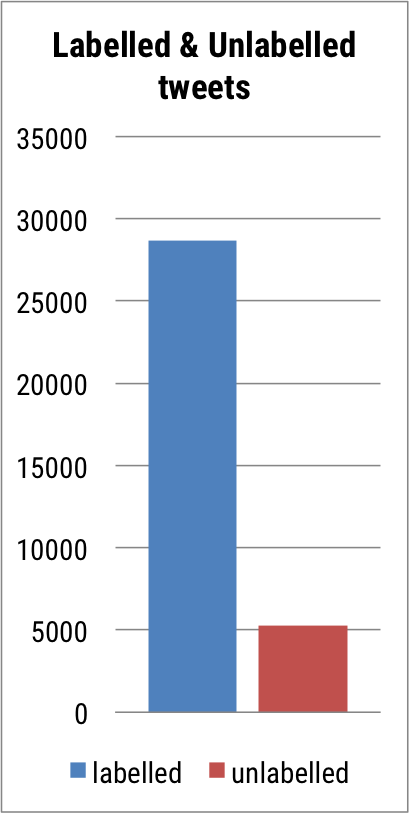
\includegraphics[width=0.95\textwidth]{EmotionLabel}
\caption{Seven days}
\label{fig:emotionLabel}
\end{subfigure}%
\begin{subfigure}{0.38\textwidth}
\centering
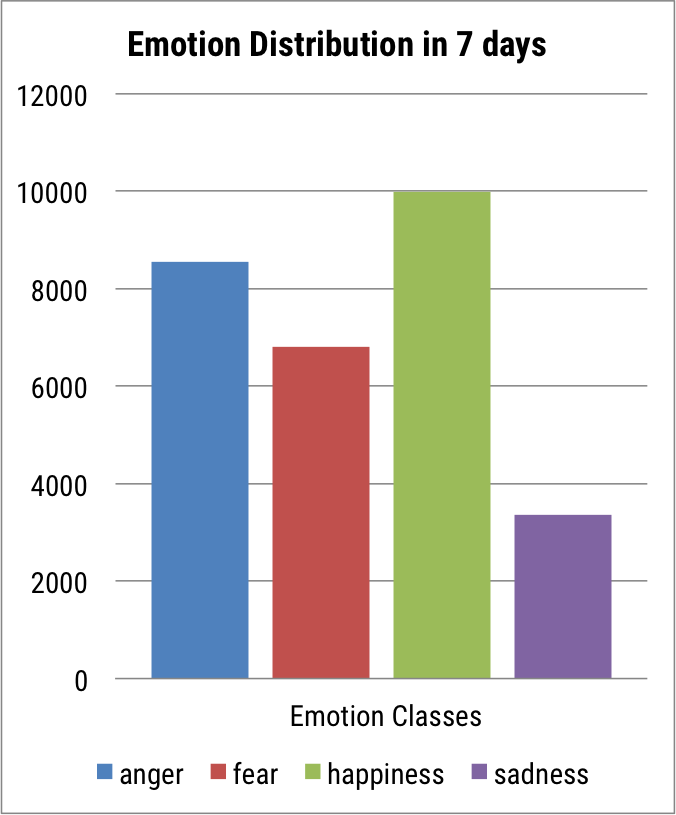
\includegraphics[width=0.95\linewidth]{EmotionDistributionWeek}
\caption{Seven days}
\label{fig:emotionDistributionWeek}
\end{subfigure}%
\begin{subfigure}{0.38\textwidth}
\centering
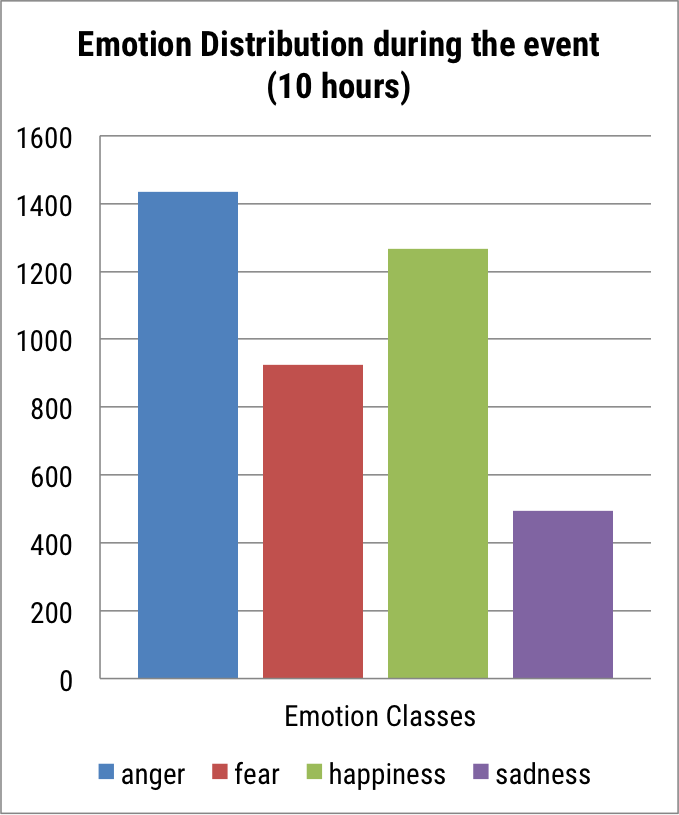
\includegraphics[width=0.95\linewidth]{EmotionDistributionEvent}
\caption{During event}
\label{fig:emotionDistributionEvent}
\end{subfigure}
\caption{The result of Emotion Analysis on the dataset (a) and the number of tweets labelled with each emotion during the event (c) and in the whole dataset of seven days (b)}
\end{figure}

As the objective of the experiment was to evaluate the framework's capability to detect the crowd types during the event, the analysis described in the next sections mainly focuses on the selected 10 hour period of the event.

\subsection{Emotion Distribution over time}
Since in our experiment, interval \(t\) was set as 15 minutes, the data was then plotted into 15 minute intervals to observe the change over time. Figure \ref{fig:instanceEvent} illustrates the change of number of tweets labelled in each emotion over time. The horizontal axis presents our focused time-line consisting of 41 time-frames. The vertical axis shows the total number of tweets labelled with a specific emotion within a time-frame. As can be noticed from the charts, angry labelled tweets reached a peak at May 3rd 9:15PM which was around the same time with the start of the boxing match. However, the increase in term of number of tweets might not be a significant lead because other emotions also reached the peaks at this time-frame.

\begin{figure}[htb!] 
\centering
\begin{subfigure}{0.5\textwidth}
\centering
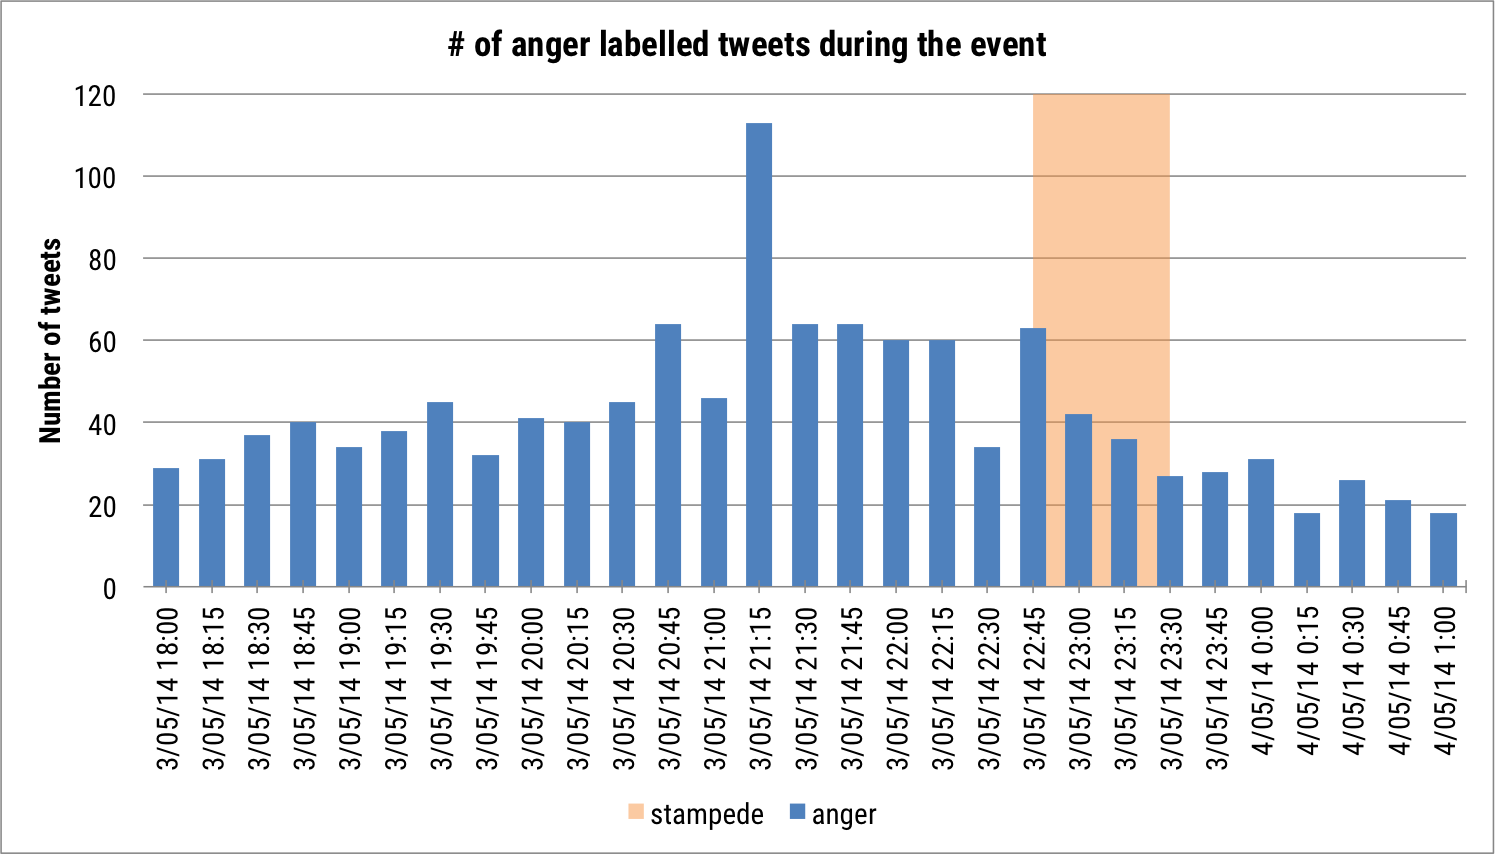
\includegraphics[width=0.99\linewidth]{AngerInstanceEvent}
\caption{anger}
\label{fig:angerInstanceEvent}
\end{subfigure}%
\begin{subfigure}{0.5\textwidth}
\centering    
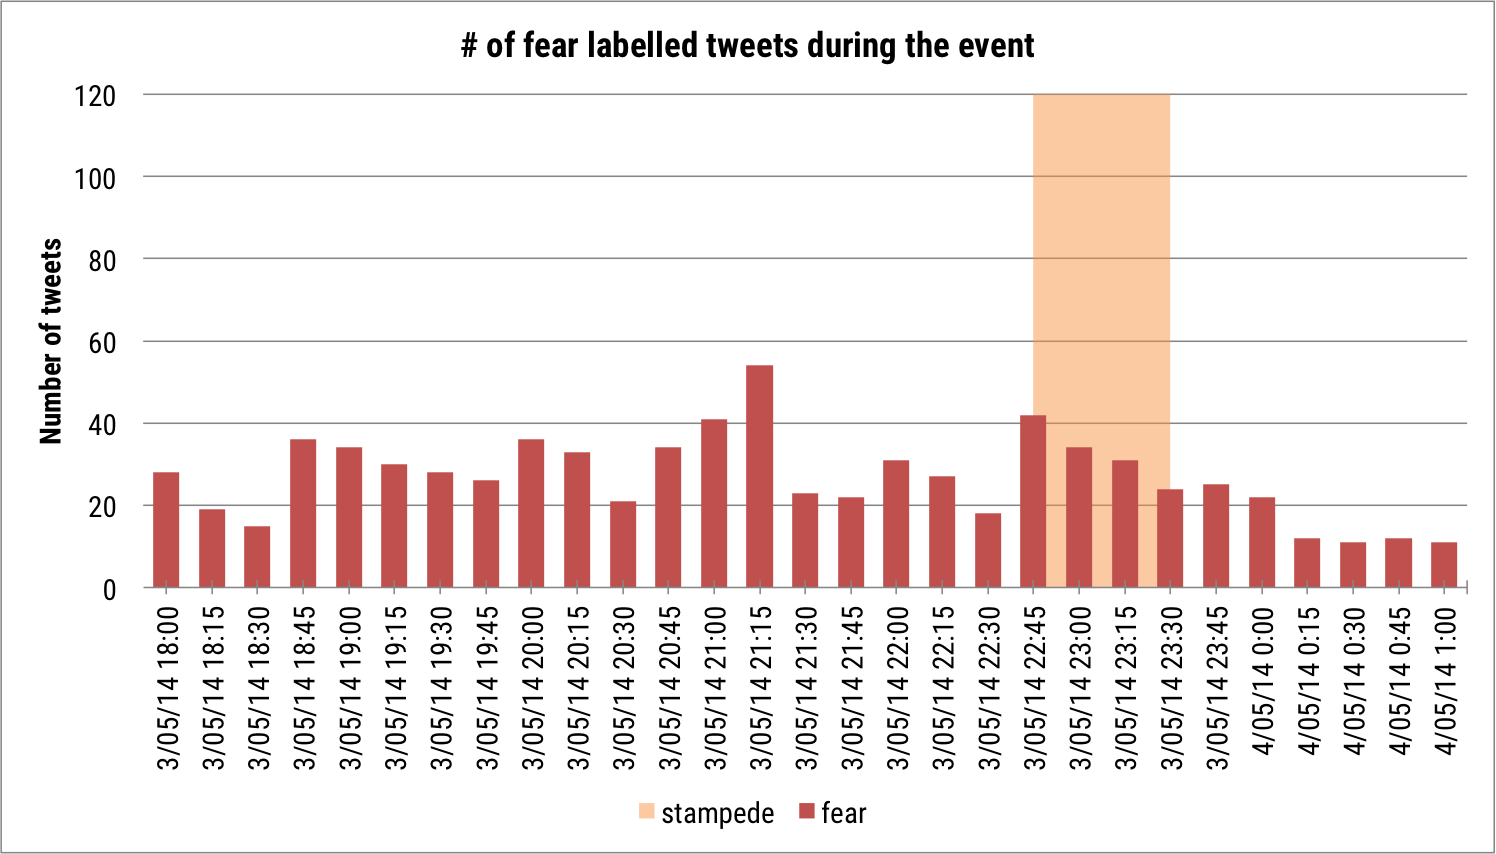
\includegraphics[width=0.99\linewidth]{FearInstanceEvent}
\caption{fear}
\label{fig:fearInstanceEvent}
\end{subfigure}

\begin{subfigure}{0.5\textwidth}
\centering    
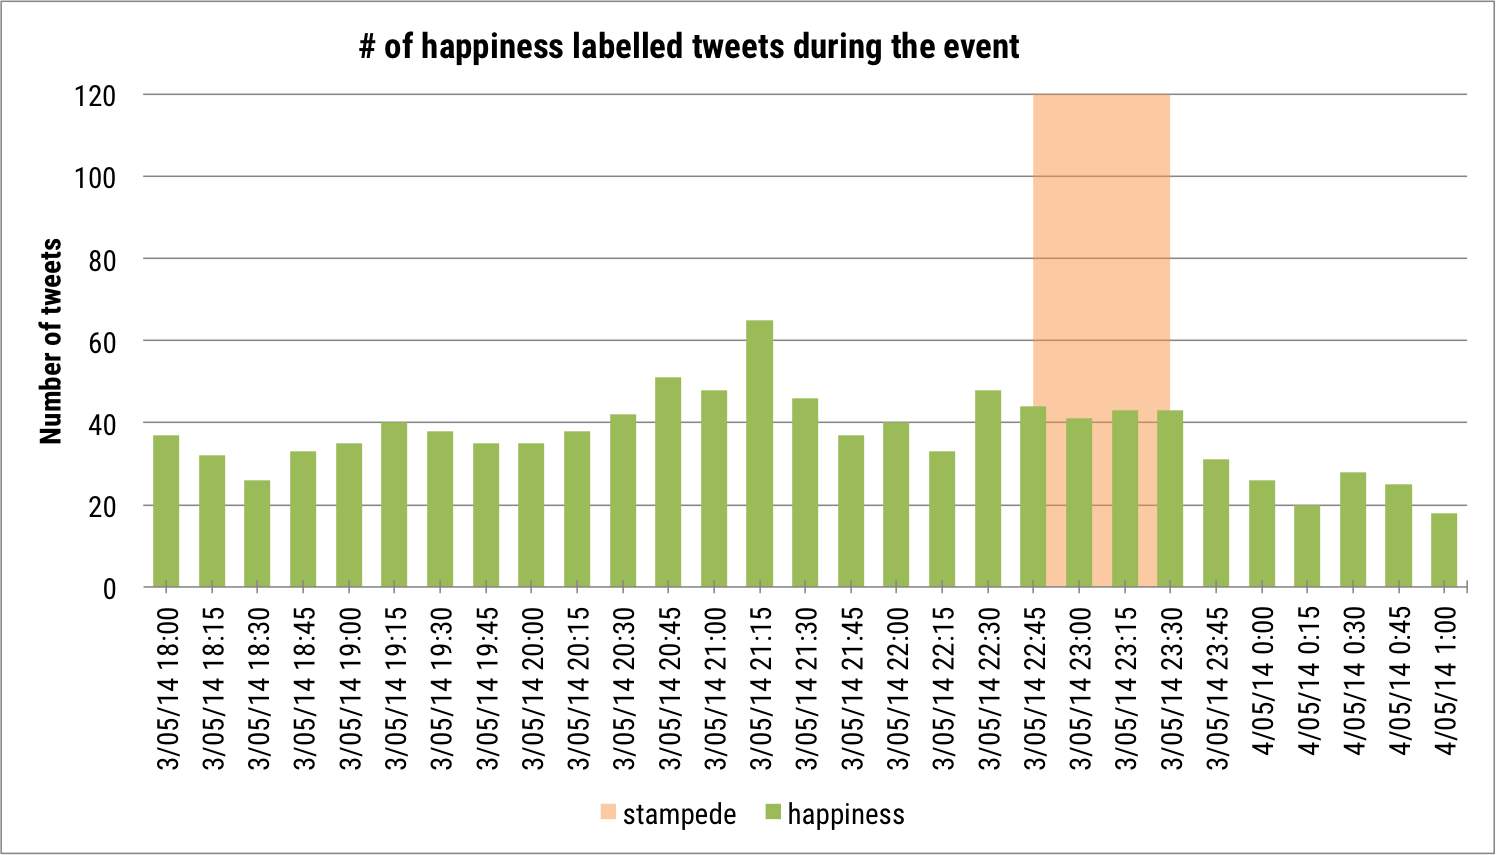
\includegraphics[width=0.99\linewidth]{HappinessInstanceEvent}
\caption{happiness}
\label{fig:happinessInstanceEvent}
\end{subfigure}%
\begin{subfigure}{0.5\textwidth}
\centering    
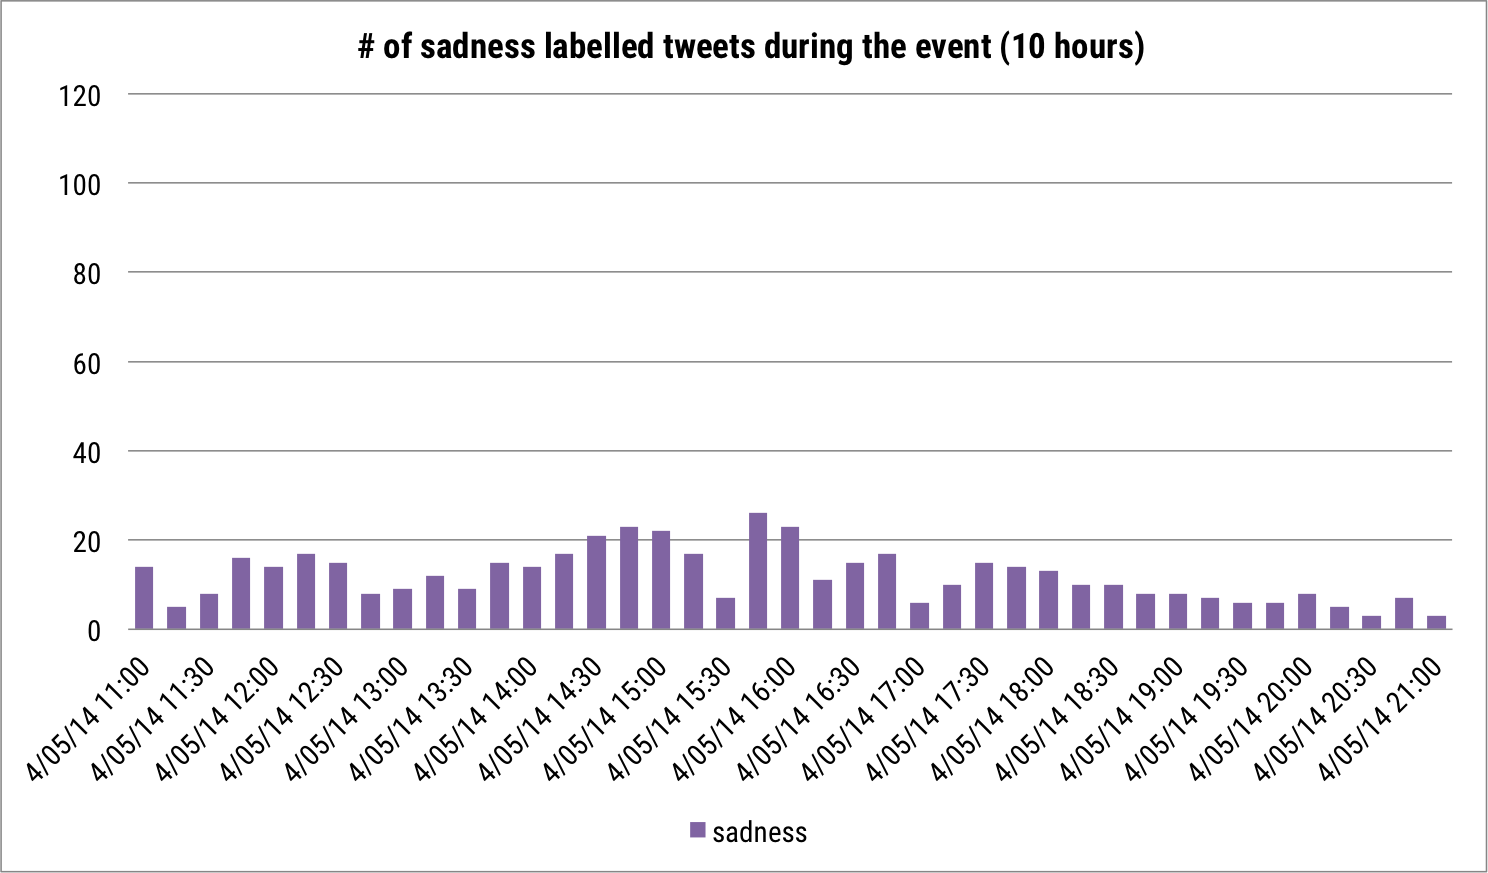
\includegraphics[width=0.99\linewidth]{SadnessInstanceEvent}
\caption{sadness}
\label{fig:sadnessInstanceEvent}
\end{subfigure}
\caption{The number of tweets labelled with anger, fear, happiness and sadness over time during the event}
\label{fig:instanceEvent}
\end{figure}

In order to reduce the effect of the increase in term of quantity, the percentage of each emotion over time was calculated according to the Formula \ref{eq:distributionEmotion} in Chapter \ref{ch:approach}. Figure \ref{fig:rateEvent} shows the emotion distribution using the percentage of tweets instead of the total number of tweets labelled with an emotion.

\clearpage
\begin{figure}[htb!] 
\centering    
\begin{subfigure}{0.5\textwidth}
\centering
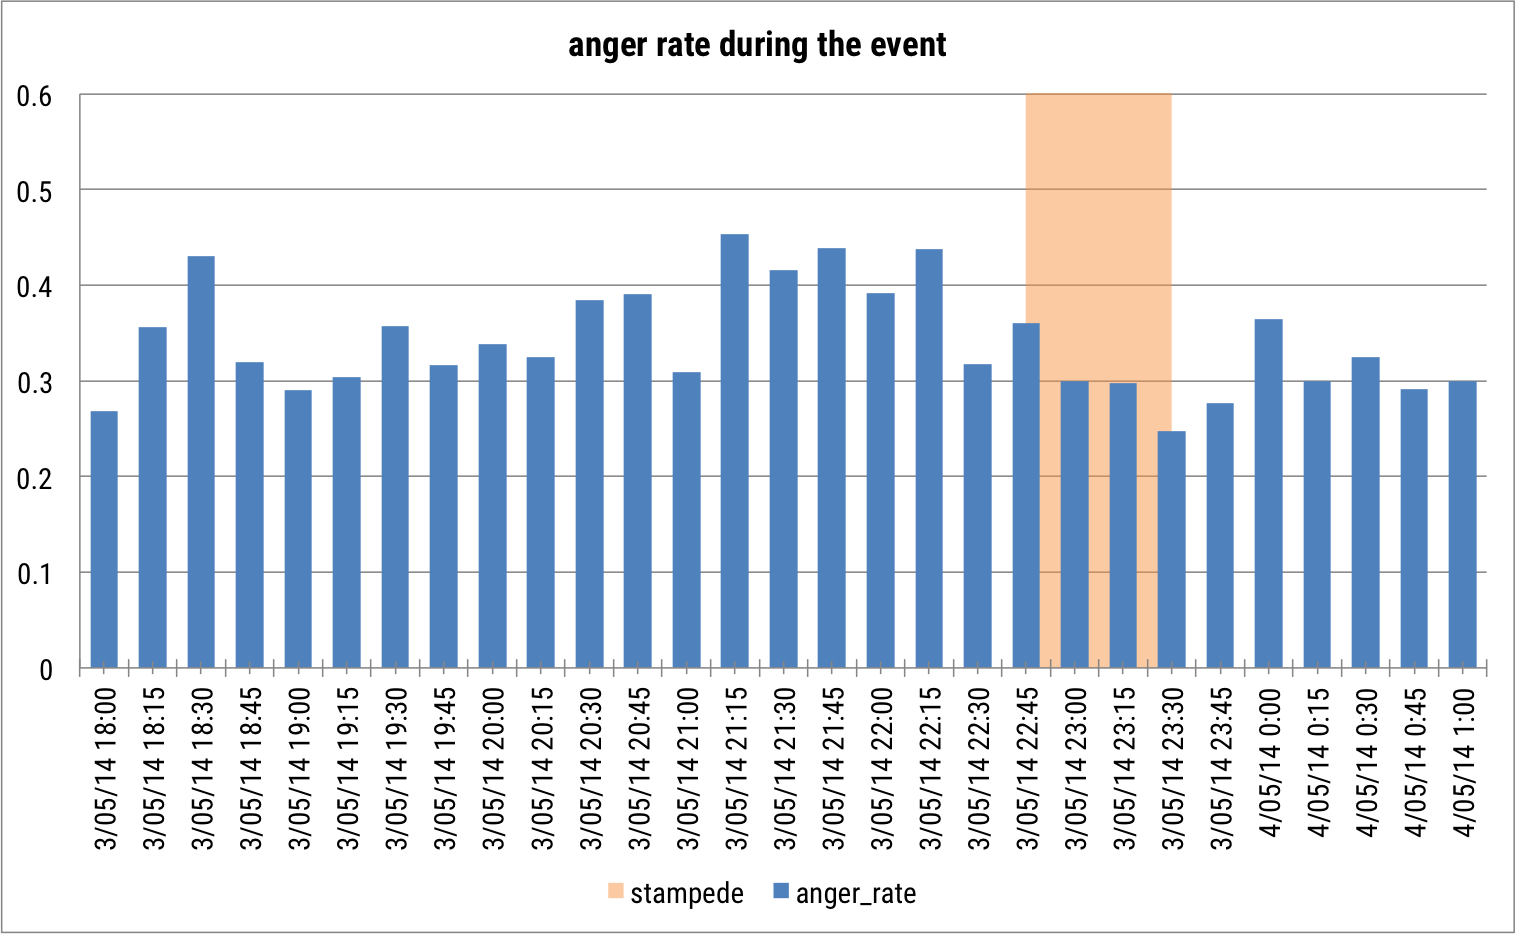
\includegraphics[width=0.99\linewidth]{AngerRateEvent}
\caption{anger}
\label{fig:angerRateEvent}
\end{subfigure}%
\begin{subfigure}{0.5\textwidth}
\centering    
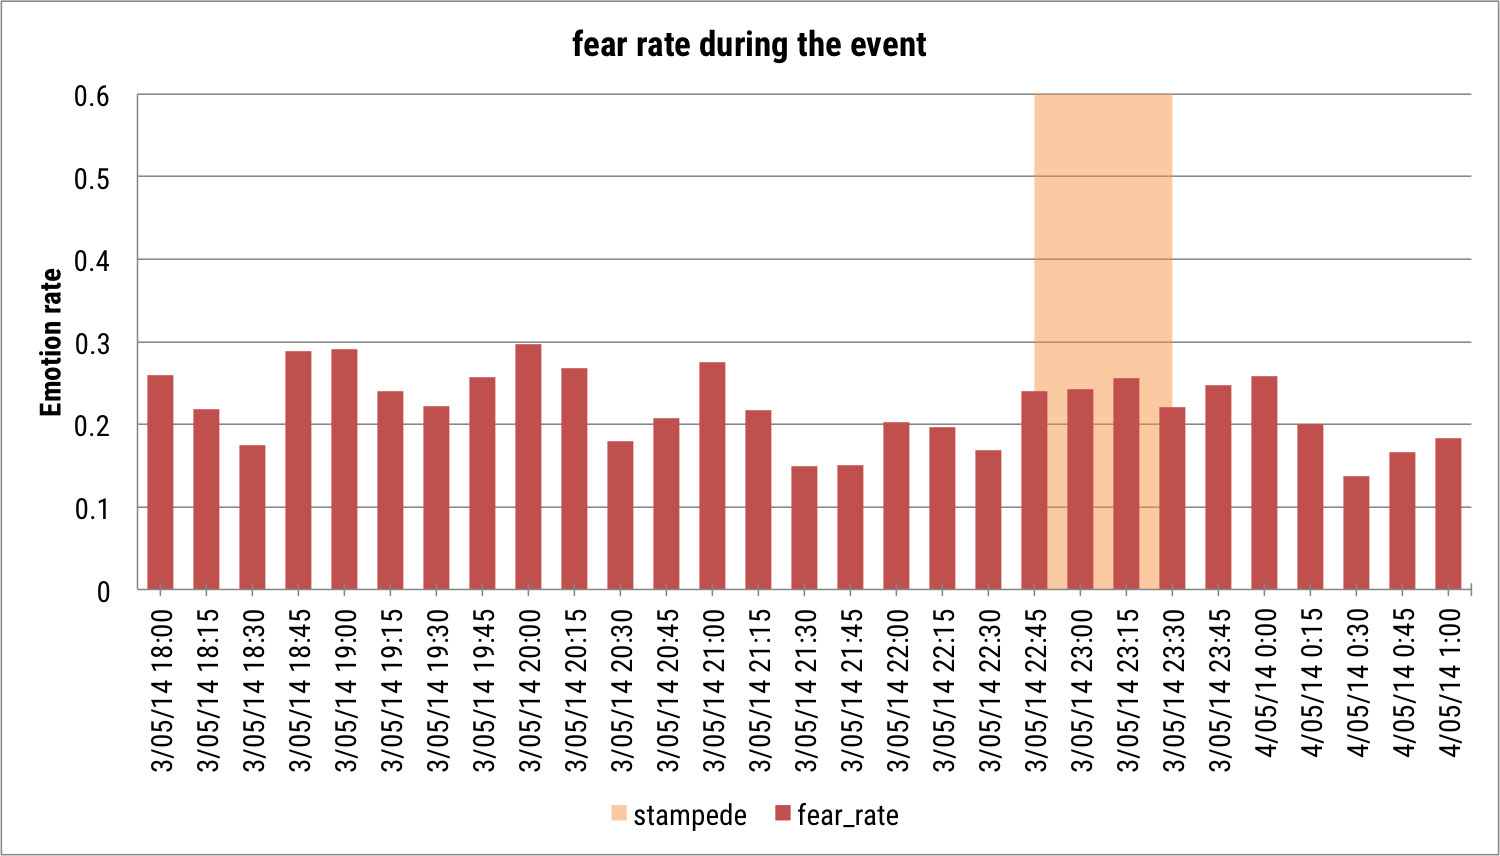
\includegraphics[width=0.99\linewidth]{FearRateEvent}
\caption{fear}
\label{fig:fearRateEvent}
\end{subfigure}

\begin{subfigure}{0.5\textwidth} 
\centering    
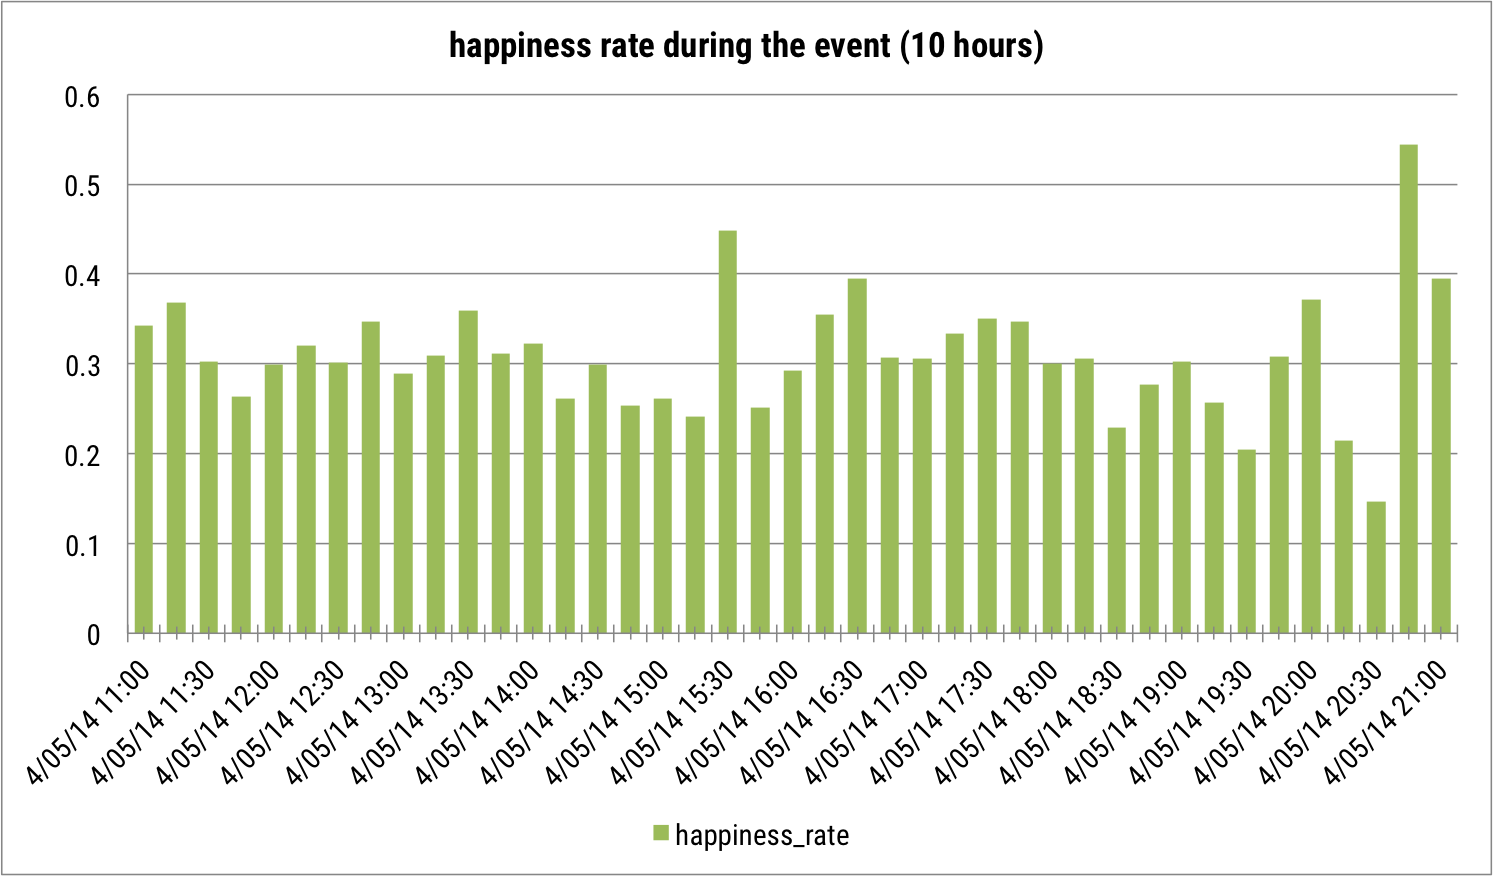
\includegraphics[width=0.99\linewidth]{HappinessRateEvent}
\caption{happiness}
\label{fig:happinessRateEvent}
\end{subfigure}%
\begin{subfigure}{0.5\textwidth}
\centering    
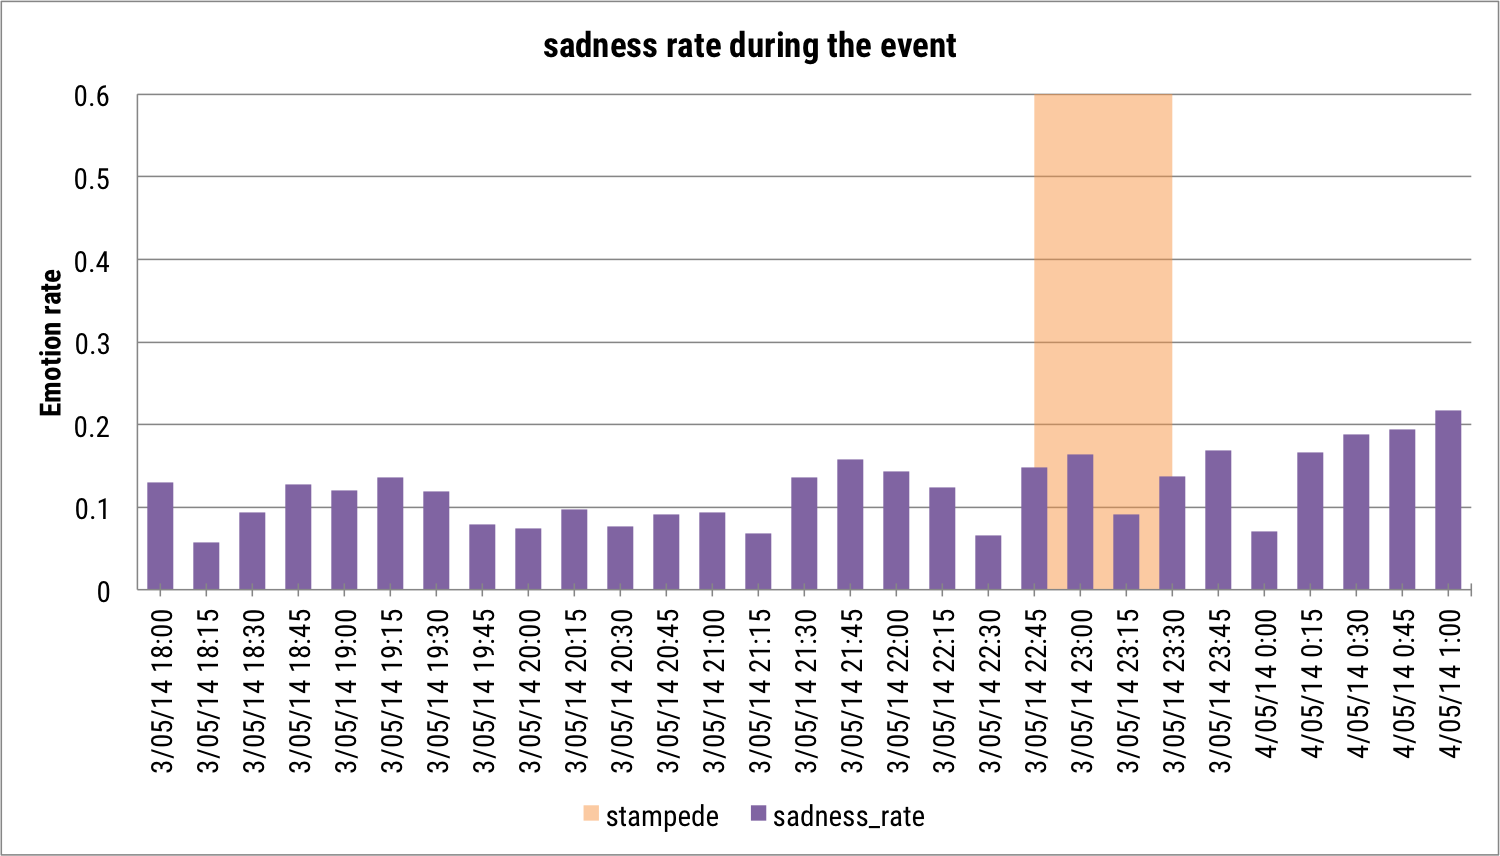
\includegraphics[width=0.99\linewidth]{SadnessRateEvent}
\caption{sadness}
\label{fig:sadnessRateEvent}
\end{subfigure}
\caption{The percentage of anger, fear, happiness and sadness over time during the event}
\label{fig:rateEvent}
\end{figure}

\subsubsection{The Normal Distribution of Emotion Rate over time}
Applying histogram to the emotion rate over time of each emotion, the distribution of the emotion rate followed the normal distribution. The majority of the values were close to the mean values forming a bell shape (Figure \ref{fig:histogramWeek}). The further a value deviates from the mean value, the less frequent its appearance is.

\begin{figure}[htb!] 
\centering    
\begin{subfigure}{0.5\textwidth}
\centering
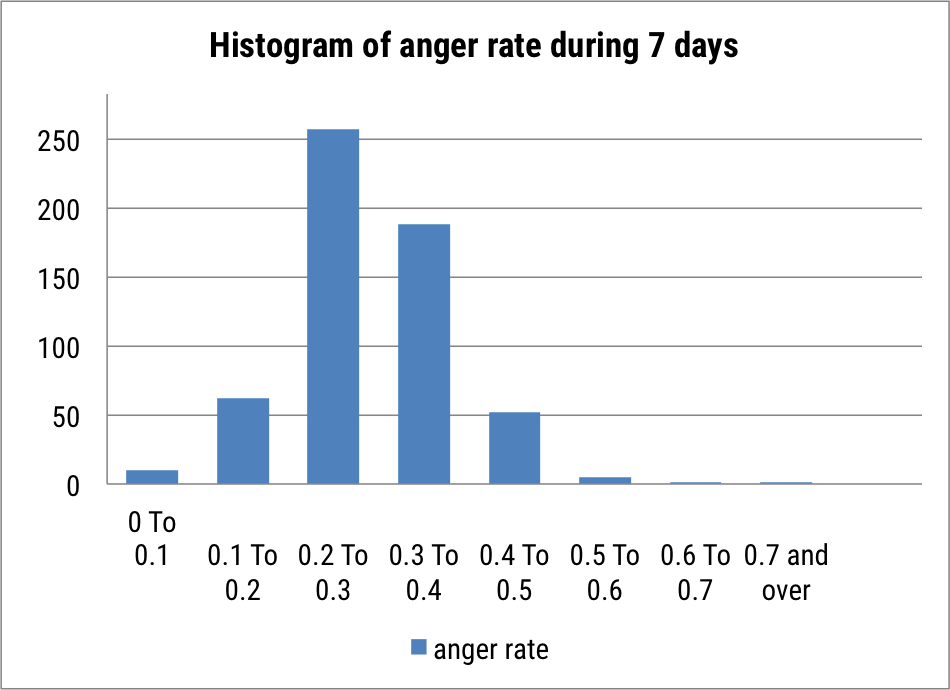
\includegraphics[width=0.8\linewidth]{HistogramAngerWeek}
\caption{anger}
\label{fig:histogramAngerWeek}
\end{subfigure}%
\begin{subfigure}{0.5\textwidth}
\centering    
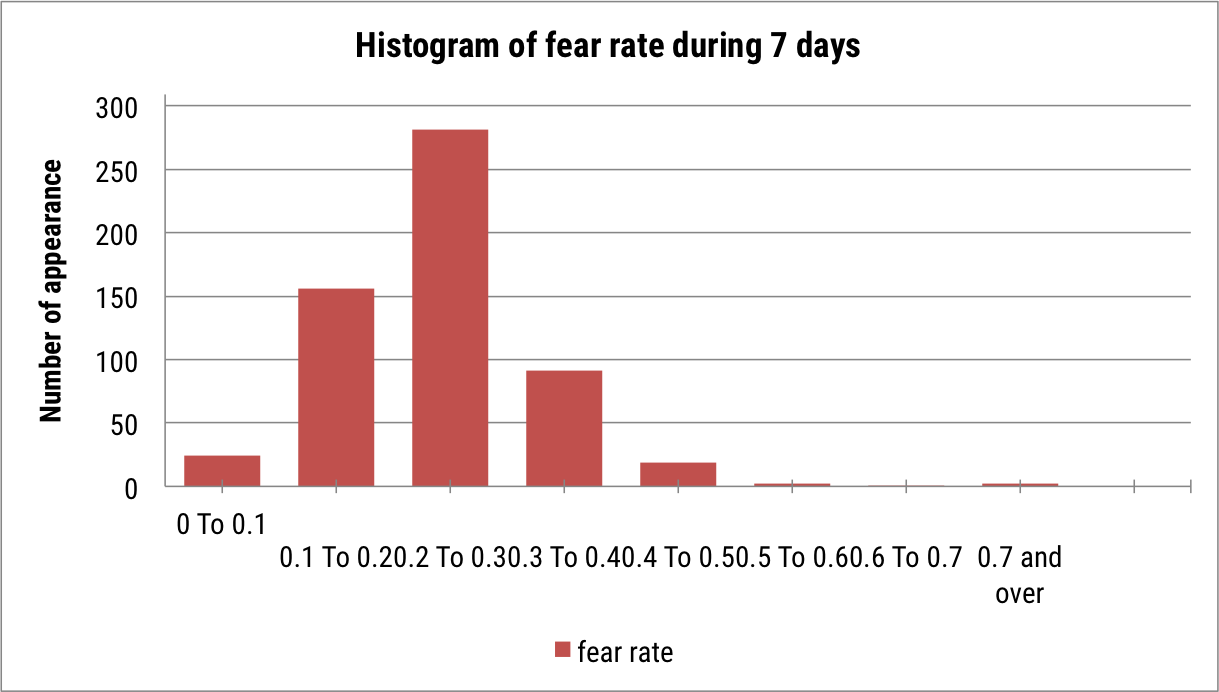
\includegraphics[width=0.8\linewidth]{HistogramFearWeek}
\caption{fear}
\label{fig:histogramFearWeek}

\end{subfigure}
\begin{subfigure}{0.5\textwidth}
\centering    
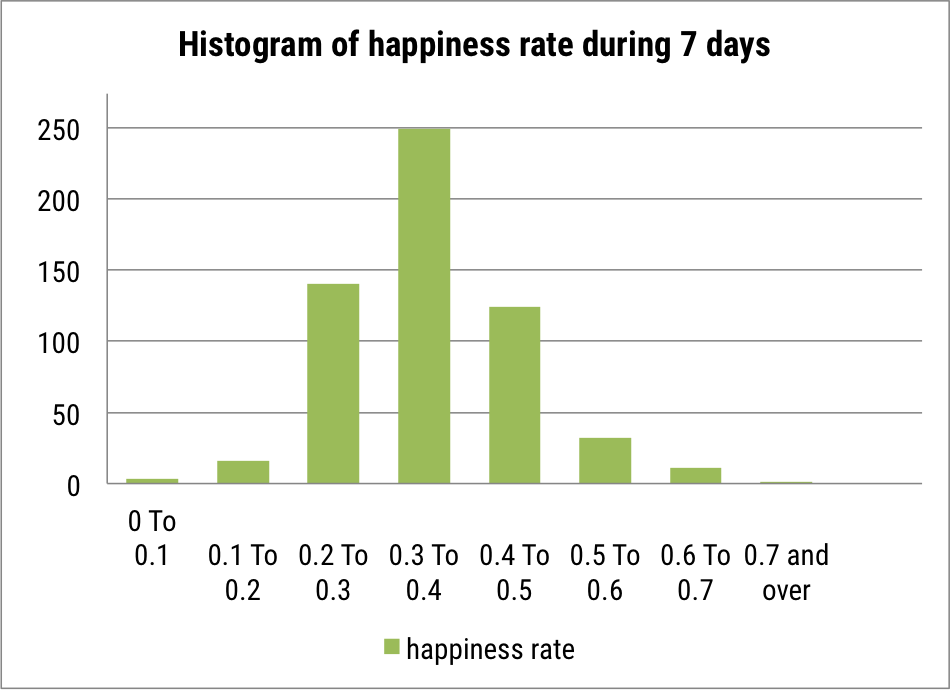
\includegraphics[width=0.8\linewidth]{HistogramHappinessWeek}
\caption{happiness}
\label{fig:histogramHappinessWeek}
\end{subfigure}%
\begin{subfigure}{0.5\textwidth}
\centering    
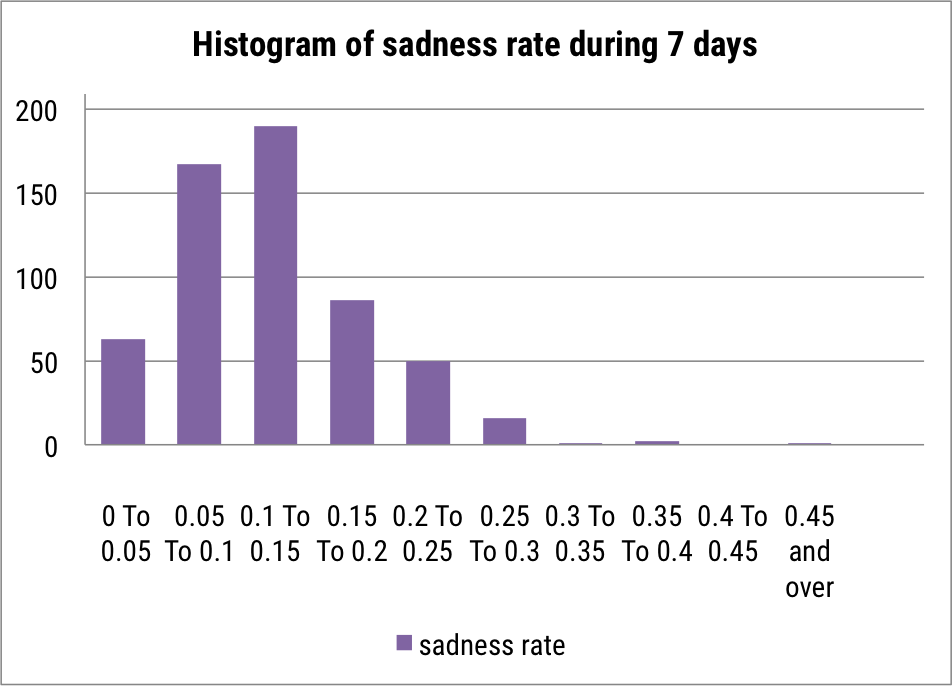
\includegraphics[width=0.8\linewidth]{HistogramSadnessWeek}
\caption{sadness}
\label{fig:histogramSadnessWeek}
\end{subfigure}
\caption{The normal distribution of anger (a), fear (b), happiness (c) and sadness (d) rate over time in the dataset}
\label{fig:histogramWeek}
\end{figure}

\subsubsection{Moving Average, Z-score and the Level of Density of an Emotion}
Set window for moving average as minus 1 hour, which means the mean value is calculate by considering 1 hour of data earlier. Set the threshold for high level of density of an emotion as z-score = 1, which means this value is higher than the mean value by one standard deviation.
\begin{figure}[htb!] 
\centering   
\begin{subfigure}{0.5\textwidth}
\centering    
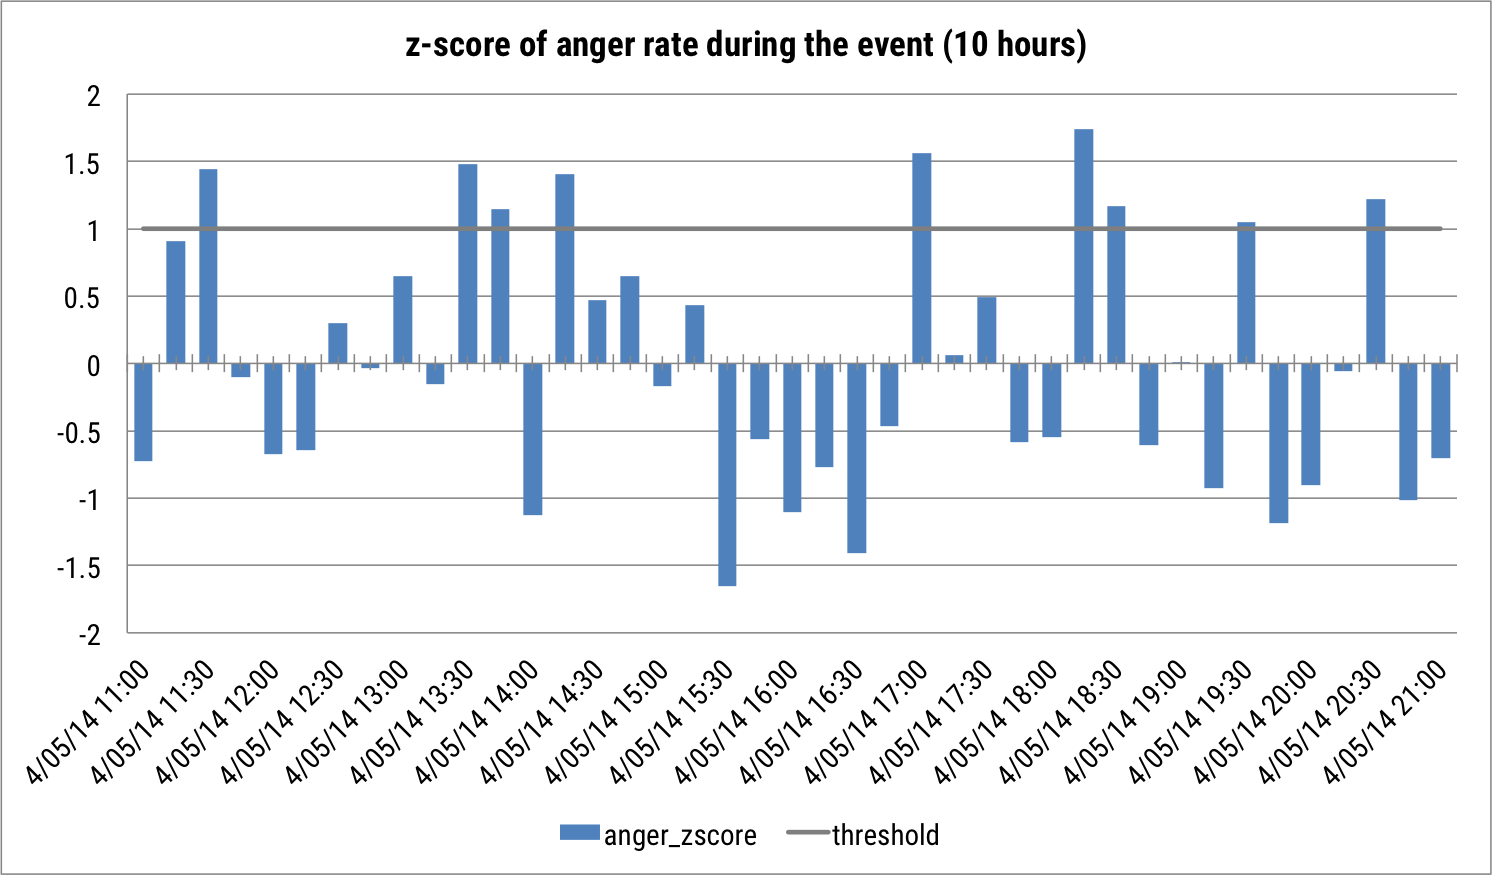
\includegraphics[width=0.99\linewidth]{AngerZscoreEvent}
\caption{anger}
\label{fig:angerZscoreEvent}
\end{subfigure}%
\begin{subfigure}{0.5\textwidth}
\centering    
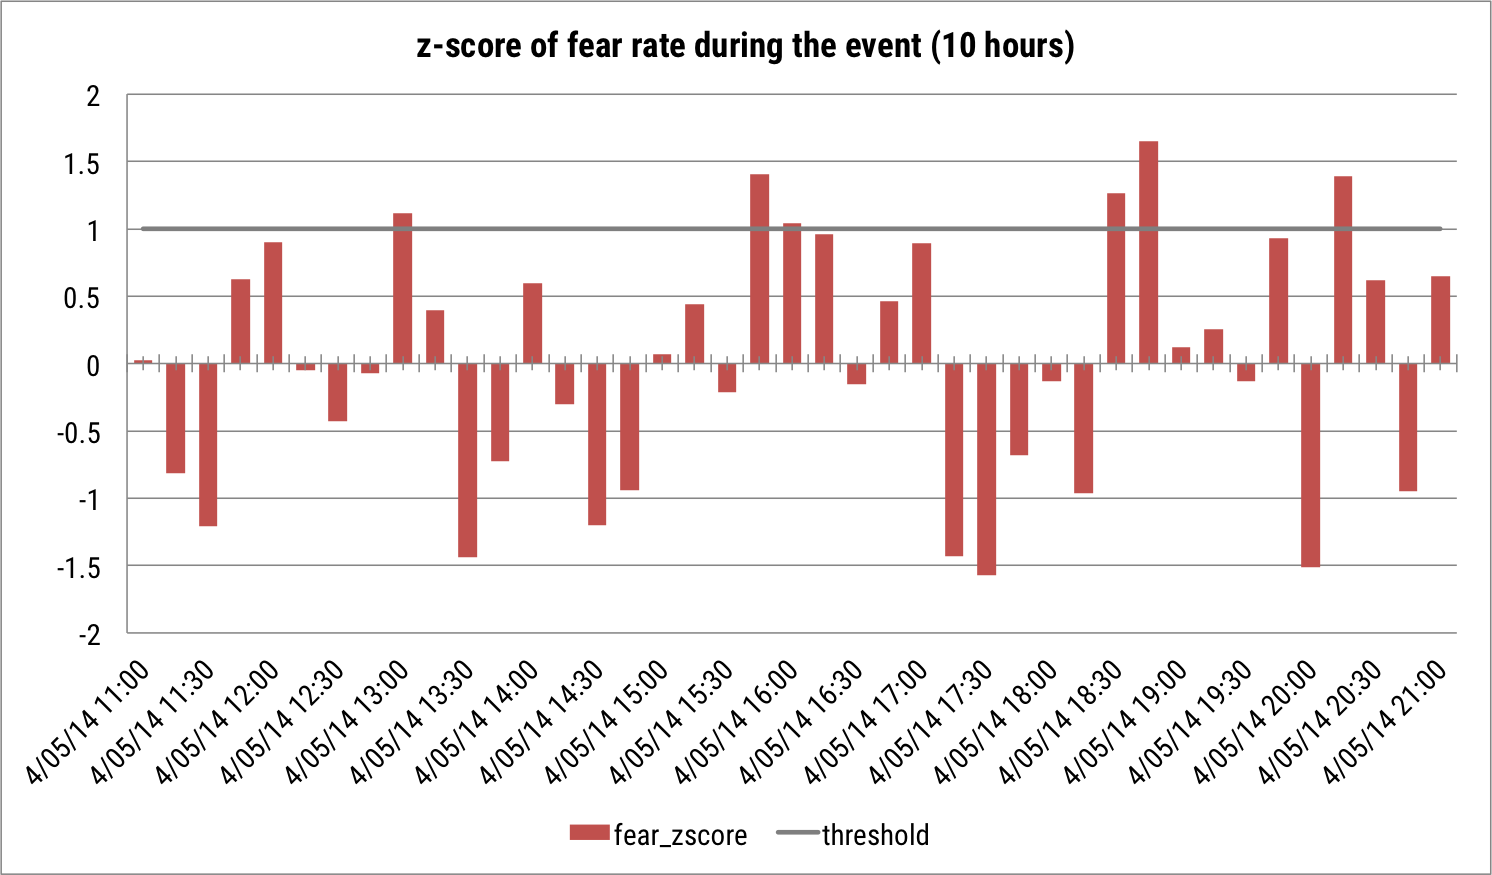
\includegraphics[width=0.99\linewidth]{FearZscoreEvent}
\caption{fear}
\label{fig:fearZscoreEvent}
\end{subfigure}

\begin{subfigure}{0.5\textwidth}
\centering    
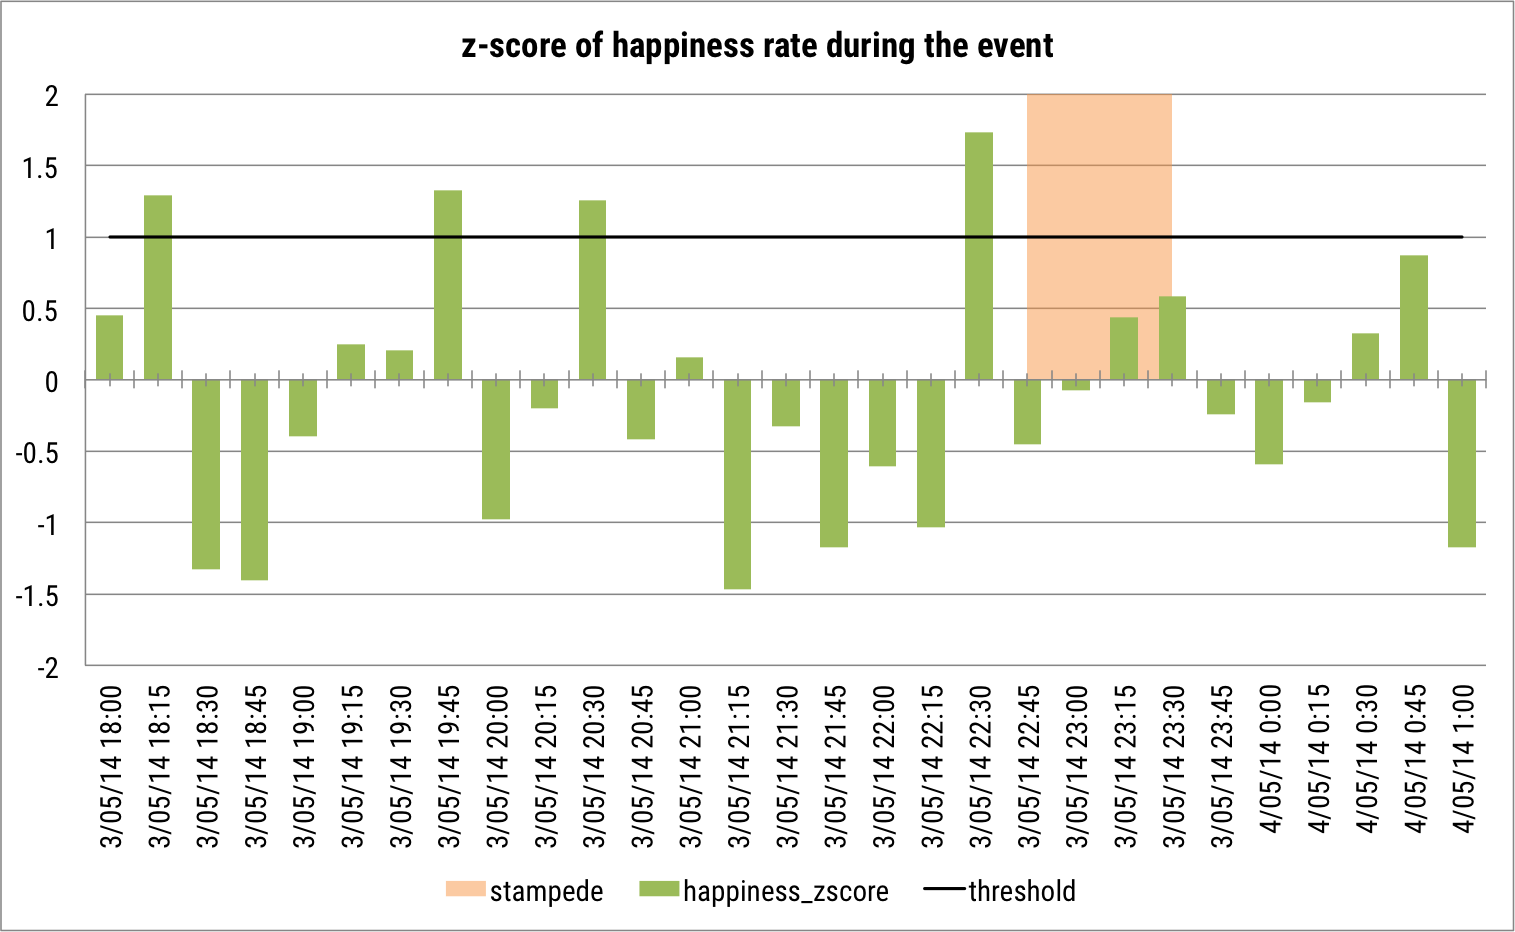
\includegraphics[width=0.99\linewidth]{HappinessZscoreEvent}
\caption{happiness}
\label{fig:happinessZscoreEvent}
\end{subfigure}%
\begin{subfigure}{0.5\textwidth}
\centering    
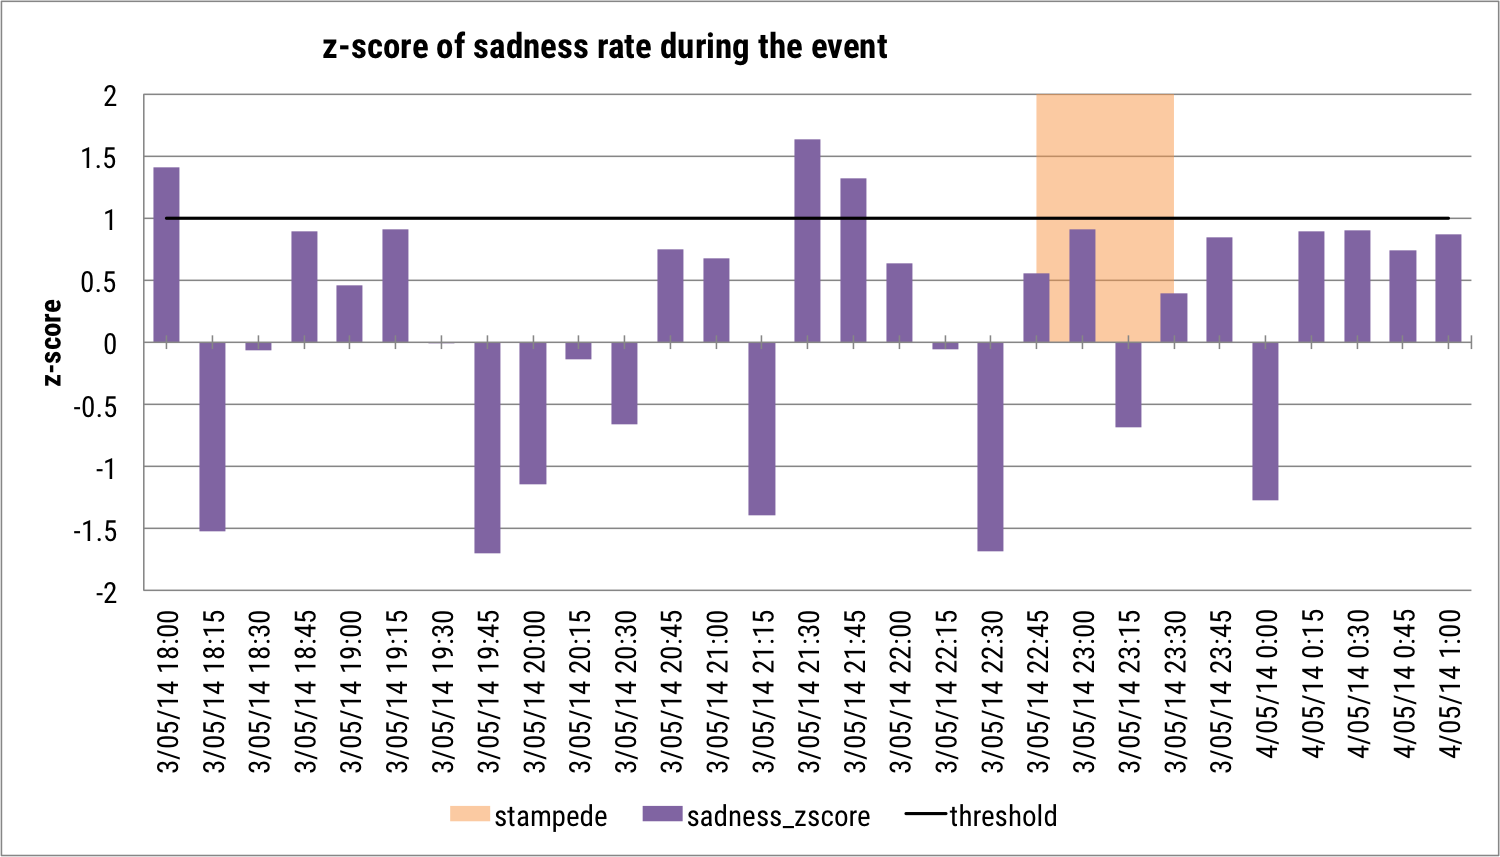
\includegraphics[width=0.99\linewidth]{SadnessZscoreEvent}
\caption{sadness}
\label{fig:sadnessZscoreEvent}
\end{subfigure}
\caption{The z-score of anger, fear, happiness and sadness rate over time during the event}
\end{figure}